
%%%%%%%%%%%%%%%%%%%%%%% file typeinst.tex %%%%%%%%%%%%%%%%%%%%%%%%%
%
% This is the LaTeX source for the instructions to authors using
% the LaTeX document class 'llncs.cls' for contributions to
% the Lecture Notes in Computer Sciences series.
% http://www.springer.com/lncs       Springer Heidelberg 2006/05/04
%
% It may be used as a template for your own input - copy it
% to a new file with a new name and use it as the basis
% for your article.
%
% NB: the document class 'llncs' has its own and detailed documentation, see
% ftp://ftp.springer.de/data/pubftp/pub/tex/latex/llncs/latex2e/llncsdoc.pdf
%
%%%%%%%%%%%%%%%%%%%%%%%%%%%%%%%%%%%%%%%%%%%%%%%%%%%%%%%%%%%%%%%%%%%


\documentclass[runningheads,a4paper]{llncs}

\usepackage{amssymb}
\setcounter{tocdepth}{3}
\usepackage{graphicx}
\usepackage{color}
\usepackage{epstopdf}

\usepackage{amsmath}
\usepackage{amssymb}

\usepackage{url}

\newcommand{\keywords}[1]{\par\addvspace\baselineskip
\noindent\keywordname\enspace\ignorespaces#1}

%shrinky
%\addtolength{\abovecaptionskip}{-3pt}
%\addtolength{\belowcaptionskip}{-5pt}
\addtolength{\textfloatsep}{-10pt}
%%\addtolength{\intextsep}{-10pt}


\begin{document}

\mainmatter  % start of an individual contribution

% first the title is needed
\title{Teaching Robots to Want}

% a short form should be given in case it is too long for the running head
\titlerunning{Teaching Robots to Want}

% the name(s) of the author(s) follow(s) next
%
% NB: Chinese authors should write their first names(s) in front of
% their surnames. This ensures that the names appear correctly in
% the running heads and the author index.
%
\author{P. Michael Furlong \and Michael Dille
}
%
\authorrunning{Furlong and Dille}
% (feature abused for this document to repeat the title also on left hand pages)

\urldef{\mailsa}\path|padraig.m.furlong@nasa.gov|

% the affiliations are given next; don't give your e-mail address
% unless you accept that it will be published
\institute{
\begin{tabular}{cp{0.1in}c}
Intelligent Robotics Group & & Robotics Institute\\
SGT / NASA Ames Research Center & & Carnegie Mellon University \\
Moffett Field, CA 94035, USA & & Pittsburgh, PA 15213, USA\\
\end{tabular} \\
\vspace{0.1in}
\mailsa
}
%\mailsa\\
%\url{http://www.tbd.com/}}

%
% NB: a more complex sample for affiliations and the mapping to the
% corresponding authors can be found in the file "llncs.dem"
% (search for the string "\mainmatter" where a contribution starts).
% "llncs.dem" accompanies the document class "llncs.cls".
%

%\toctitle{Foraging in Territories Strange}
%\tocauthor{Furlong \and D.}
\maketitle


\begin{abstract}
% Max 150 words
This paper presents a new algorithm for autonomous on-line exploration in unknown environments.  The objective of the algorithm is to free robot scientists from extensive preliminary site investigation while still being able to collect meaningful data.  We simulate a common form of exploration task for an autonomous robot involving sampling the environment at various locations and compare performance with a simpler existing algorithm that is also denied global information.  The result of the experiment shows that the new algorithm has a statistically significant improvement in performance with a significant effect size for a range of costs for taking sampling actions.
\keywords{foraging, active learning, planetary exploration}
\end{abstract}

%% main text
\section{Introduction}
\label{sec:intro}

Human scientists have become accustomed to such luxuries as breathing, eating
and drinking, and enduring atmospheric and gravitational forces that do not
vary significantly from ``1.''  Consequently, robots have become our scientific
surrogates as we peer into the depths of the ocean or into our solar
neighbourhood.  High-latency and low-bandwidth communication to these regions limits the situational awareness and reaction times of the scientists controlling such robots.  For this reason it is important to increase the ability of robotic explorers to independently make in-mission decisions.

A common exploration activity is remote sensing, in which a robot is tasked with collecting sensor data by sampling the environment at various locations.  The nature of many specialized sensors often employed for activities such as biological collection and spectral mapping requires long energy-intensive sampling durations or the activation of single-use collection canisters.  Given constraints on mission length and payload capacity coupled with limited remote operator awareness, some autonomy in sampling location selection is vital to mission productivity and success.

Currently fielded robots either depend highly on their operators for objectives or plan with considerable global knowledge.  Operating in such conditions constrains them to rely on either remote human decision-making (requiring often impractical levels of situational awareness) or significant amounts of prior scouting, obviating the need to send a robotic agent.  These limitations are mirrored in existing literature, which fails to provide principled reasoning about what to investigate \emph{in situ} without such reliances.

This paper presents an algorithm that addresses one common instance of such missions, in which objects or areas found in the environment lie within some respective class that is readily sensed, and each class possesses some underlying data distribution (e.g. spectral response or biochemical composition) that can only be sensed by activating the expensive specialized sensor.  The overall goal is to estimate the underlying distribution of each class with maximal accuracy.

For scientific realism and general applicability, no global information such as a prior map of sampling opportunities is available, sensing opportunities are assumed to arise nondeterministically (e.g. from classes present along a pre-determined trajectory or as currents draw objects past the robot), and the robot cannot return to objects it did not choose to sample.  Thus, the problem can be thought of as a stream of sensing opportunities providing varying reward (information about the underlying distribution of a class), each requiring a decision to sample or move on.

The use of this algorithm is motivated by observations of human and animal behavior, exemplified by geologists making decisions about investigating local phenomena without prior access to detailed maps, in which they are able to effectively choose between sampling from materials in front of them or moving on to potentially more profitable sampling locations.  While these decisions may not be globally optimal, they do demonstrate an ability that is lacking in current exploration robots: to make decisions to stop and engage with the environment or to continue traveling in the hope of finding more informative sampling locations.




%Why did I do the work?
%	Robots exploring the world right now either depend highly on their controllers to give them objectives or they are planning with some global knowledge.  Operating in these kinds of conditions puts constraints on robot exploration opterations by relying on either humans to make decisions or a significant amount of scouting.
%	Relying on humans to make decisions means that remote operators require considerable bandwidth to acquire sufficient situational awareness.  Conducting sufficient reconnaissance to make good decisions often obviates the need to send a robotic agent.
%	What is lacking in the literature are robots that make decisions about what to investigate \emph{in situ} without reliance on humans and without necessarily having global knowledge.
	
	
%What were the central motivations and hypotheses?
%	Animals, e.g. human geologists, make decisions about investigating phenomena in the world without necessarily having access to high resolution satellite imagery.  Despite this lack they are able to chose between sampling from materials in front of them and moving on to determine more profitable sampling locations.
%	While these decisions may not be globally optimal they do demonstrate an ability that is lacking from exploration robots: to make decisions to stop and engage with the environment or to continue travelling in the hopes of finding more informative sampling locations.




\section{Background}
\label{sec:background}

Automating experiment design is not without precedent.  Kristine Smith started the field of optimal experiment design in 1918 \cite{smith1918standard}.
It is only recently that robots have been employed to conduct scientific exploration autonomously \cite{wagner2001science},\cite{king2004functional}.  We will discuss below is how current robot scientists reliance on global information prevents them from operating in truly unknown environments.  Additionally, we will cover how previous approaches in sequential decision making from statistics do not necessarily reflect the settings that autonomous robots encounter in the real world.


	Who else has done what?

- Evidence that humans make (approximately) rational decisions (we over and under estimate low and high probabilities)

	- Design of experiments has led to (amongst other things) multi-armed bandit models of sequential experiment design.
	- See also maximum entropy sampling
	- See also mutual information sampling.
- Also consider active learning solutions (they all end up being the same anyway)

	- Robotics research has made robots that conduct exploration, but the only ones that make decisions about whether to investigate something or not do one of three things:
	1. match templates.
	2. seek improbable things.
	3. Engage in opportunistic science - they do something if they have the time.  They don't override human mission objectives.

	1 and 2 say nothing about the information content of the material under investigation.
	3 does not have the level of autonomy that we need for truly long-term or remote operations.

	How?

	What have we previously done:
	- D.R. Thompson's work
	- Only looking at satellite imagery.  Good but not sufficient.
	- Trey's work
	- Using POMDPs not scalable to a planet.
	- Mine. Where does my previous work fall short?
- Not bayesian (not a big deal?)
	- Still has the problem on knowing the number of sampling opportunities remaining.

\subsection{The Secretary Problem}

		- Secretary problem
			- They know what the value of their choice is, in many cases.
			- They know how many candidates there are.
			- We have rates of arrival, they just have a queue.
			- While our sampling time cost implies an upper bound on the number of 
			candidates we don't have a lower bound necessarily.

\subsection{Multi-armed bandits}

		- Multi-armed bandit
			- Assumes you can access any arm at any time
			- Many settings don't have a switching cost between arms.
			- Gittins showed that if you have a switching cost and diminishing returns you can solve the problem.
			- We say is we will be randomly assigned an arm and a switching cost.

\subsection{Optimal Foraging}

	- Work in the 1970's about foraging.  About making value judgements.
		- Key point from Charnov's work is that there has to be diminishing returns
		for extracting from a field (specifically towards an asymptote)
		- Different from our setting is that diminishing your reward in one area 
		contributes to diminishing your reward elsewhere. It isn't like picking
		apples off one tree, and finding a new tree with unpicked apples.


	- Piroli 1999 - has come up with a very similar formulation as the one that 
		Mike and I came up with.
		- Something to consider is that we only get to take one sample per patch 
			because of science differentiation requirements (i.e. RP can't have 
			samples closer than 10cm to each other, maybe as far as 1m)
		- We could also incorporate the different cost it takes to identify things 
			in the scene.
		- We also have different times between patches.
		- Should it come to multiple contexts then we have the contextual bandit 
			problem
				- This means that we could keep different distributions of classes per 
					environment.


\subsection{Science Autonomy}

	- Thompson, Asher Bender and Stephane Williams Group
			- making selections based on maps.  
			- Maximum entropy/mutual information smapling.
			- They assume global knowledge, we don't have that.  It is reasonable
			in many settings of interest, can reduce cost.


	- Previous work in robotic exploration is either dependent on global information or it does not make reasoned decisions about the rest of the world and the sampling opportunities that are immediately available to it.
			- opportunistic science only takes advantage of what is immediately availble to the robot and with surplus sampling budget.
			- whoi and mbari follow set patterns (which is fine, the lawnmower is a good and noble thing) but they use an arbitrary threshold to make the decision to sample or not.  They do not take into account the rest of the environment.


	- Dudek and co., using novelty to slow down the driving an collect more data.
		- Ditto their other paper.

\subsubsection{Our Prior Work}
		- Apply optimal foraging, specifically Charnov's marginal value theorem
		model of foraging to the problem of science autonomy* in the following setting:	
			- Limited sampling budget
			- Attempting to learn distributions not acquire quantities of some object.
			- Trying to learn information objectively without an objective. 
			- Can't know the reward until you sample.
			- It's a fusion of bandits and foraging.  The fact that we are focusing on gaining information gives us diminishing returns which lets us use 
			- Don't have access to all the arms at any given time, which is what makes it a foraging problem.
			- Don't have the choice of what objects you encounter.

As seen above real robots may not be able to predict the rewards they will earn from their actions and have to deal with unreliable arrival rates for sampling opportunities.  These are concerns that are not modelled in typical sequential experiment selection algorithms such as the Multi-armed bandit or secretary problems.  This motivates the problem setting used in this paper, and that describe in detail in the following section.

\section{Method}
\label{sec:method}

The decision making agents in this paper are tested on several randomly
generated transects.  They are repeatedly presented with an object to sample
and have to make the choice to either take a sample or continue travelling
along the transect.  Like the Robbins' secretary problem the agents are not
permitted to backtrack to avail of a previous opportunity.


Figure \ref{fig:transect} gives an example of a simulated transect. As we can
see there are sampling opportunities of different types scattered along the
path that the robot travels along.  

\begin{figure}[htpd!]
	\centering 
	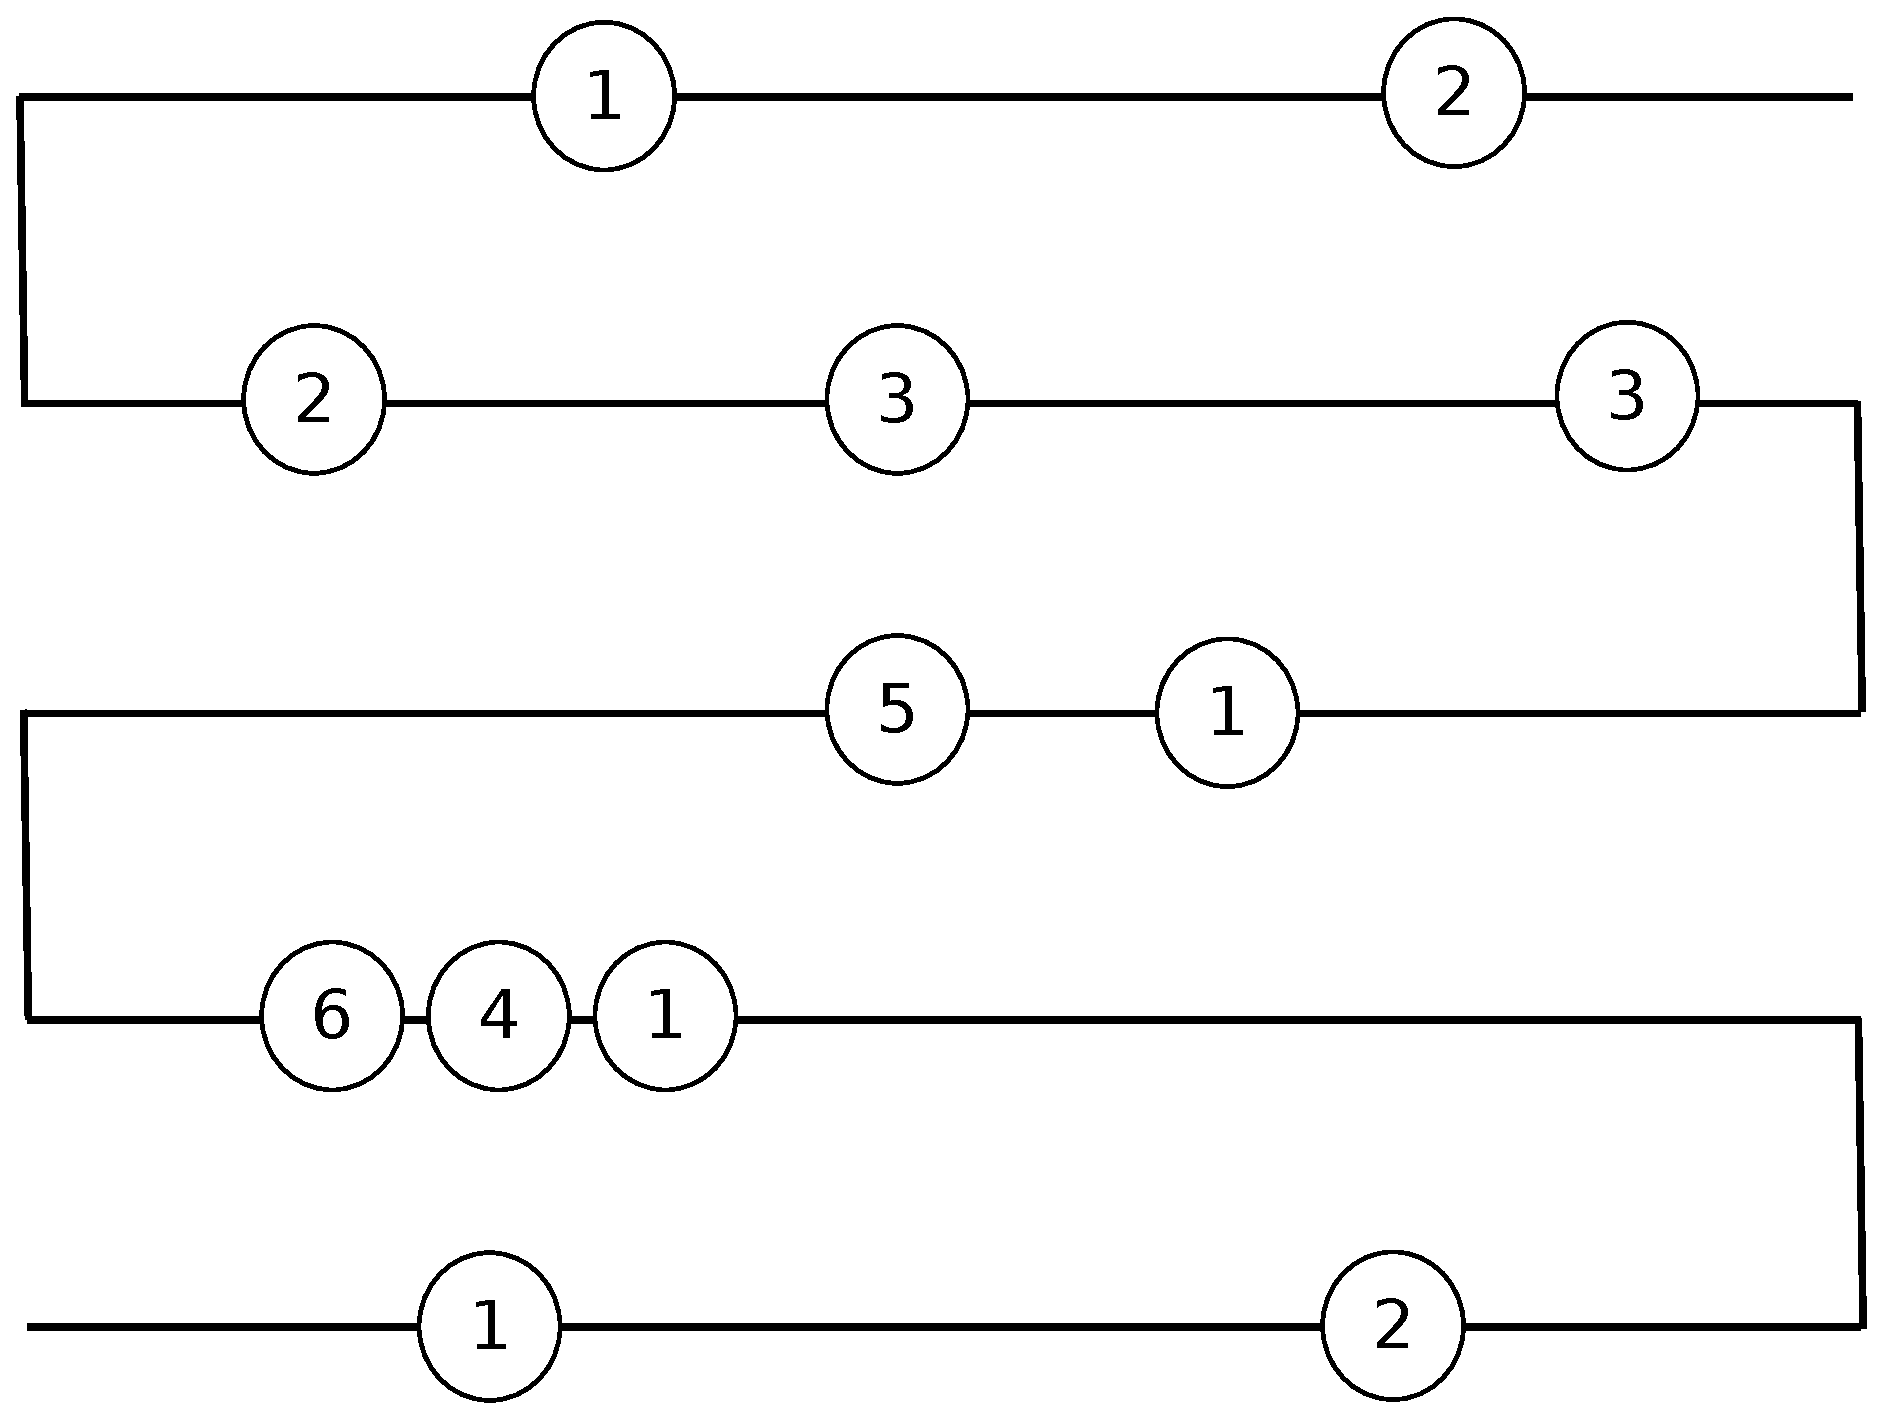
\includegraphics[width=0.8\textwidth]{transect}
	\caption{A cartoon illustrating a transect a robot might be encountering and how samping opportunities of different types may be distributed along it.  In the field the robot would start at one end of the path and follow it to the other end.  There is one path that the rover may follow across the terrain resulting in it encountering different types of sampling opportunities.}
	\label{fig:transect}
\end{figure}


The primary objective of the robot is to learn distributions behind different
classes of objects.  For example they may be the probability distribution
governing the density of sub surface microbial life in different classes of
soil.  Previous work have identified that texture information can successfully
classify different types of soil material \cite{paper_that_trey_and_thompson_cite_in_their_image_return_paper}.  
We imagine that the classes of objects in
this research could correspond to those soil classes.



\subsection{Experiment}

The experiment presented in this paper is a modification of the experiments
presented in \cite{furlong2014sequential} and \cite{furlong2014budgeting}.  In the
prior work agents were equipped with limited sampling budgets.  In this
experiment the agents have an unlimited capacity to take samples, but the time
to take the sample is non-zero and there is an overall limit on the duration of
the mission.

As with the previous experiments the agents are not permitted to back track in
the hopes of getting a better opportunity.  The primary reason is to constantly
drive the robot to the end of its exploration mission.  Coverage is an
important part of exploration and permitting.  Additionally making decisions
between a current opportunity, a hypothetical future, and any number of
previously seen but unsampled opportunities is considered a more complex
problem and outside the scope of this paper.

In the experiment there are six different kinds of objects the agent may
encounter.  They each have their own arrival rate and their appearance along
the transect are generated with a poisson process.  In this paper the arrival
rates of the different sampling opportunities do not change over the course of
the experiment.  While this is almost certainly not the case for long range
traversals like those seen in the Life in the Atacama Desert Project it is a
reasonable approximation for shorter-range traverses.

\subsection{Algorithms}

	% This is only relevant in the larger work.
	% - figure method.3: texture cam, raw image and texture labelled image.

	The experiment builds on prior work.  Here we present three algorithms that are being testing on the simulated transect described above.

\subsubsection{Uniform Sampling}

The Uniform Sampling algorithm attempts to distribute the number of samples it
can collect evenly between the different types of objects present on the
transect.  This is chosen because it was a robustly successful algorithm, as
seen in the prior work \cite{furlong2014sequential} and \cite{furlong2014isairas}.

The Uniform Sampling algorithm does not consider the time remaining in the
transect, nor the time to complete sampling.

\subsubsection{Foraging}

The foraging algorithm is an attempt to maximize the productivity of the learning agent along the transect.  We attempt to maximize the number of bits learned per unit time.

The reward for sampling a class is an analog for the definition of surprise as
defined by the Koch et al {cite papers}.  Koch looked at the change in the
distribution that resulted in a Bayesian update.  Because this work uses a
non-parametric kernel density estimation we compare
$\log\left(\frac{\hat{p}(x|D\cup \left\{x\right\})}{\hat{p}(x|D)}\right)$.  To
be compatiable with optimal foraging algorithms, specifically the Marginal
Value Theorem of Charnov \cite{charnov1973optimal} the reward function must
have dimishing returns.  In the case of information update the Bayes Factor
will eventually converge to approximately 1, likewise our estimated empirical
bayes factor.  We take the log of this approximation such that it converges to
zero as more samples are collected.


	- figure method.2: The reward function as samples are given to it, for two or three different distributions.

	- Combining foraging models with bandit literature 
		- The previous work on foraging assumed an inherent value to
			options that the agent cared about.  Specifically, energy stored up.
		- We use a valuation model taken from bandit literature.  
		- We use the reward function from Koch's attention models
		- We use the decision making process from foraging. 
		- We add the concept of multi-arrival rate things, awareness of time limits.
	- Previous work had a limit on the number of samples it could take
		- We realized that the actual quantity that limits the exploration process
			is time.
		- By limiting the time and (in this case) relaxing the limit on sample sizes we more accurately deal with productivity.  
	- This experiment models a type of prospecting where the number of samples isn't limited but they do take time. 
	- To that end we are looking at productivity.

	-  This experiment is more akin to contextual bandits.  
	- The image represents a context, the NIRVSS 
	- Apply texturecam classification of a scene, as the context
	- the choice is to sample or continue

	- Productivity 



\section{Results}
\label{sec:results}


- Figure results.1: Overall error at the end of the trial with unlimited sampling and without weighing by the rarity (1/prob of occurrence) of the class
- Figure results.2: overall error at the end of the trial with unlimited sampling and with weighing by the rarity of the class
- Figure results.3: Overall performance when combining limited time and limited sample budgets.



\section{Conclusion}
\label{sec:conclusion}

\begin{quote}
	Foraging algorithms are the bo-shizzle spank.
	\\
	-- Benjamin Disraeli 
\end{quote}


\bibliographystyle{splncs03}
\bibliography{merged}

\appendix

\end{document}
